\documentclass{beamer}

\usepackage[utf8]{inputenc}
\usepackage{verbatim}
\usepackage{bm} % for correct font and emphasis in formulation max/min
\usepackage{multirow}

% For ignoring margins in slides.
\newcommand\Wider[2][3em]{%
\makebox[\linewidth][c]{%
  \begin{minipage}{\dimexpr\textwidth+#1\relax}
  \raggedright#2
  \end{minipage}%
  }%
}

% Necessary for formulation layout workaround.
\newcommand{\pushright}[0]{\hskip \textwidth minus \textwidth}
\makeatletter
\newcommand{\specialcell}[1]{\ifmeasuring@#1\else\omit$\displaystyle#1$\ignorespaces\fi}

\AtBeginSection[]
{
  \begin{frame}[noframenumbering,plain]
    \frametitle{Outline for ``\currentsection''}
    \tableofcontents[
    currentsubsection,
    hideothersubsections,
    sectionstyle=show/shaded
    ]
  \end{frame}
}

% Allows for refering to the current section name
\newcommand{\currentsection}{}
\newcommand{\mysection}[1]{\renewcommand{\currentsection}{#1}\section{#1}}

\beamertemplateballitem
\usetheme{Antibes}
	\usecolortheme[RGB={120,0,0}]{structure}
	\setbeamertemplate{blocks}[rounded][shadow=true]
%\setbeamertemplate{footline}{\insertframenumber/\inserttotalframenumber}
	\setbeamerfont{page number in head/foot}{size=\large}
	\setbeamertemplate{footline}[frame number]
	\setbeamercovered{transparent=5}
	\setbeamertemplate{navigation symbols}{}
	% To number the references.
	\setbeamertemplate{bibliography item}{\insertbiblabel}

% used to avoid counting references as extra slides
\newcommand{\backupbegin}{
   \newcounter{framenumberappendix}
   \setcounter{framenumberappendix}{\value{framenumber}}
}
\newcommand{\backupend}{
   \addtocounter{framenumberappendix}{-\value{framenumber}}
   \addtocounter{framenumber}{\value{framenumberappendix}}
}

\usepackage{algorithm}
\usepackage[noend]{algpseudocode}

\newcommand{\dslidefs}{\footnotesize}

\usepackage{tikz}
% Define transparent elements
\setbeamercovered{invisible}
\newcommand{\semitransp}[2][35]{\color{fg!#1}#2\color{fg!100}}
\newcommand{\drawhvector}[5]{
	\edef \origin {#1}
	\edef \xmax {#2}
	\edef \rs {(#3,#4)}
	\edef \scale {#5}
	\foreach \x in {0,...,\xmax}{
		\draw [shift={\origin}] (\x,0) rectangle +\rs;
		\node [scale=\scale, shift={\origin}, font=\LARGE] at (\x + 0.5, 0.5) {\(\x\)};
	}
}
\newcommand{\drawhvectornotext}[5]{
	\edef \origin {#1}
	\edef \xmax {#2}
	\edef \rs {(#3,#4)}
	\edef \scale {#5}
	\foreach \x in {0,...,\xmax}{
		\draw [shift={\origin}] (\x,0) rectangle +\rs;
		%\node [scale=\scale, shift={\origin}, font=\LARGE] at (\x + 0.5, 0.5) {\(\x\)};
	}
}
\newcommand{\drawhvectorfill}[6]{
	\edef \origin {#1}
	\edef \xmax {#2}
	\edef \rs {(#3,#4)}
	\edef \scale {#5}
	\edef \filling {#6}
	\foreach \x in {0,...,\xmax}{
		\draw [shift={\origin},fill=\filling] (\x,0) rectangle +\rs;
		%\node [scale=\scale, shift={\origin}, font=\LARGE] at (\x + 0.5, 0.5) {\(\x\)};
	}
}
\newcommand{\drawaxis}[2]{
	\edef \xmax {#1}
	\edef \ymax {#2}
	\draw [<->, thick] (\xmax,0) -- (0,0) -- (0,\ymax);
	\node [below, font=\small] at (\xmax/2, 0) {weight};
	\node [rotate=90, above, font=\small] at (0,\xmax/2) {profit};
}
\newcommand{\dominate}[3]{
	\edef \xx {#1}
	\edef \yy {#2}
	\edef \xmax {#3}
	\draw [dashed] (\xx, 0) -- (\xx,\yy) -- (\xmax,\yy);
}

% 12-color safe palette for color blindness
% http://mkweb.bcgsc.ca/colorblind/palettes.mhtml#page-container
\definecolor{jam}{RGB}{159,1,98}
\definecolor{creepers}{RGB}{0,159,129}
\definecolor{barbie}{RGB}{255,90,175}
\definecolor{aquamarine}{RGB}{0,252,207}
\definecolor{french}{RGB}{132,0,205}
\definecolor{dodger}{RGB}{0,141,249}
\definecolor{capri}{RGB}{0,194,249}
\definecolor{plum}{RGB}{255,178,253}
\definecolor{carmine}{RGB}{164,1,34}
\definecolor{crimson}{RGB}{226,1,52}
\definecolor{outragerous}{RGB}{255,110,58}
\definecolor{spark}{RGB}{255,195,59}

% Change the spacing in a 'table of contents'/outline
\usepackage{etoolbox} % allows patching macros
\makeatletter
\patchcmd{\beamer@sectionintoc}{\vskip1.5em}{\vskip0.5em}{}{}
\makeatother

\newif\ifplacelogo % flag to disable logo
\placelogotrue % displays logo unless set to false

\begin{document}

\title{An enhanced formulation for guillotine 2D cutting problems}
\author{Henrique Becker\\[2\baselineskip] \small Advisor: Luciana S. Buriol\\Co-Advisor: Olinto Araujo}
\logo{\ifplacelogo
\includegraphics[scale=0.2]{inf}\fi}
\date{Friday, December 11, 2020}

{
	\setbeamertemplate{footline}{}
	\begin{frame}[noframenumbering]
	\titlepage
	\end{frame}
}

% LAST THING TODO: create a list of topics and copy it between each section
{
	\setbeamertemplate{footline}{}
	\begin{frame}[noframenumbering]
	\frametitle{Outline}
	\tableofcontents[hideallsubsections]
	\end{frame}
}

% Colors: jam, creepers, barbie, aquamarine, french, dodger, capri, plum,
% carmine, crimson, outragerous, spark

\mysection{Introduction}
\subsection{The Problem}
\frame{\frametitle{Objective Function}
\center
The Guillotine 2D Knapsack (G2KP) maximizes the profit obtained from cutting pieces from a single large `original plate'.

\def\kx{0.200}
\def\ky{0}
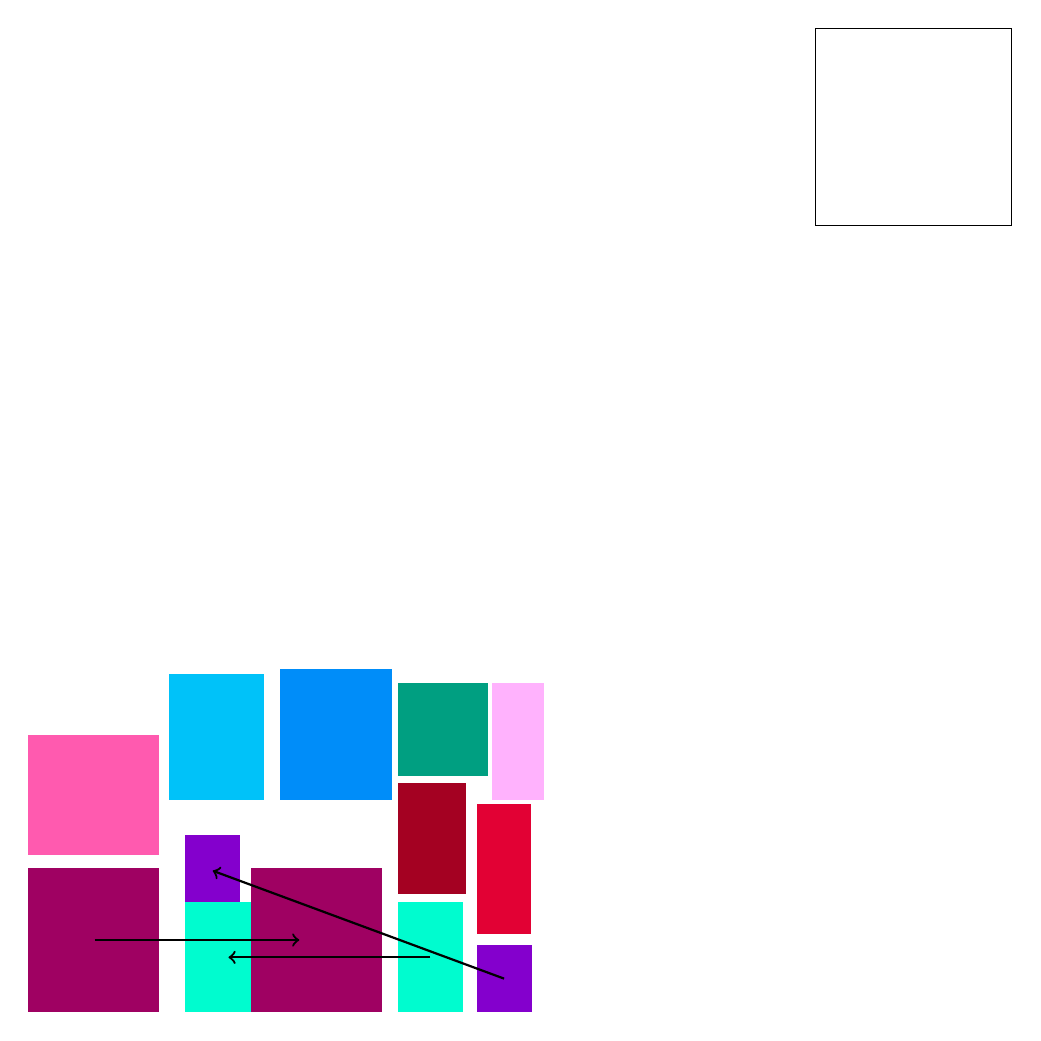
\begin{tikzpicture}[scale=10]

\fill[aquamarine] (0.470,0) rectangle +(0.083, 0.140);
\onslide<3-4>{\fill[aquamarine] (0.200,0) rectangle +(0.083, 0.140);}

\fill[french] (0.570,0) rectangle +(0.070, 0.086);
\onslide<3-4>{\fill[french] (0.200,0.140) rectangle +(0.070, 0.086);}

\fill[jam] (0,0) rectangle +(0.167, 0.184);
\onslide<3-4>{\fill[jam] (0.283,0) rectangle +(0.167, 0.184);}

\onslide<2-3>{\draw[thick,->] (0.605, 0.043) -- (0.235,0.180);} % french violet
\onslide<2-3>{\draw[thick,->] (0.511, 0.070) -- (0.255,0.070);} % aquamarine
\onslide<2-3>{\draw[thick,->] (0.085, 0.092) -- (0.345,0.092);} % jam

\fill[barbie] (0,0.200) rectangle +(0.167, 0.152);
\fill[creepers] (0.470,0.300) rectangle +(0.114, 0.118);
\fill[dodger] (0.320,0.270) rectangle +(0.143, 0.166);
\fill[capri] (0.180,0.270) rectangle +(0.120, 0.160);
\fill[plum] (0.590,0.270) rectangle +(0.066, 0.148);
\fill[carmine] (0.470,0.150) rectangle +(0.087, 0.141);
\fill[crimson] (0.570,0.10) rectangle +(0.069, 0.165);

\draw[black] ++(\kx, \ky) +(0,0) rectangle +(0.250, 0.250);
%\draw[dashed, thick, black] ++(\kx, \ky) +(0.083,0) -- +(0.083, 0.250);
%\draw[dashed, thick, black] ++(\kx, \ky) +(0,0.140) -- +(0.083, 0.140);
%\draw[dashed, thick, black] ++(\kx, \ky) +(0,0.226) -- +(0.083, 0.226);
%\draw[dashed, thick, black] ++(\kx, \ky) +(0.070,0.140) -- +(0.070, 0.250);
%\draw[dashed, thick, black] ++(\kx, \ky) +(0.083,0.184) -- +(0.250, 0.184);
\end{tikzpicture}
}

\frame{\frametitle{Guillotine Cuts}
\center
``every cut always go from one side of a plate to other; a cut never stops or starts from the middle of a plate''

\center
\def\kx{0.300}
\def\ky{0}
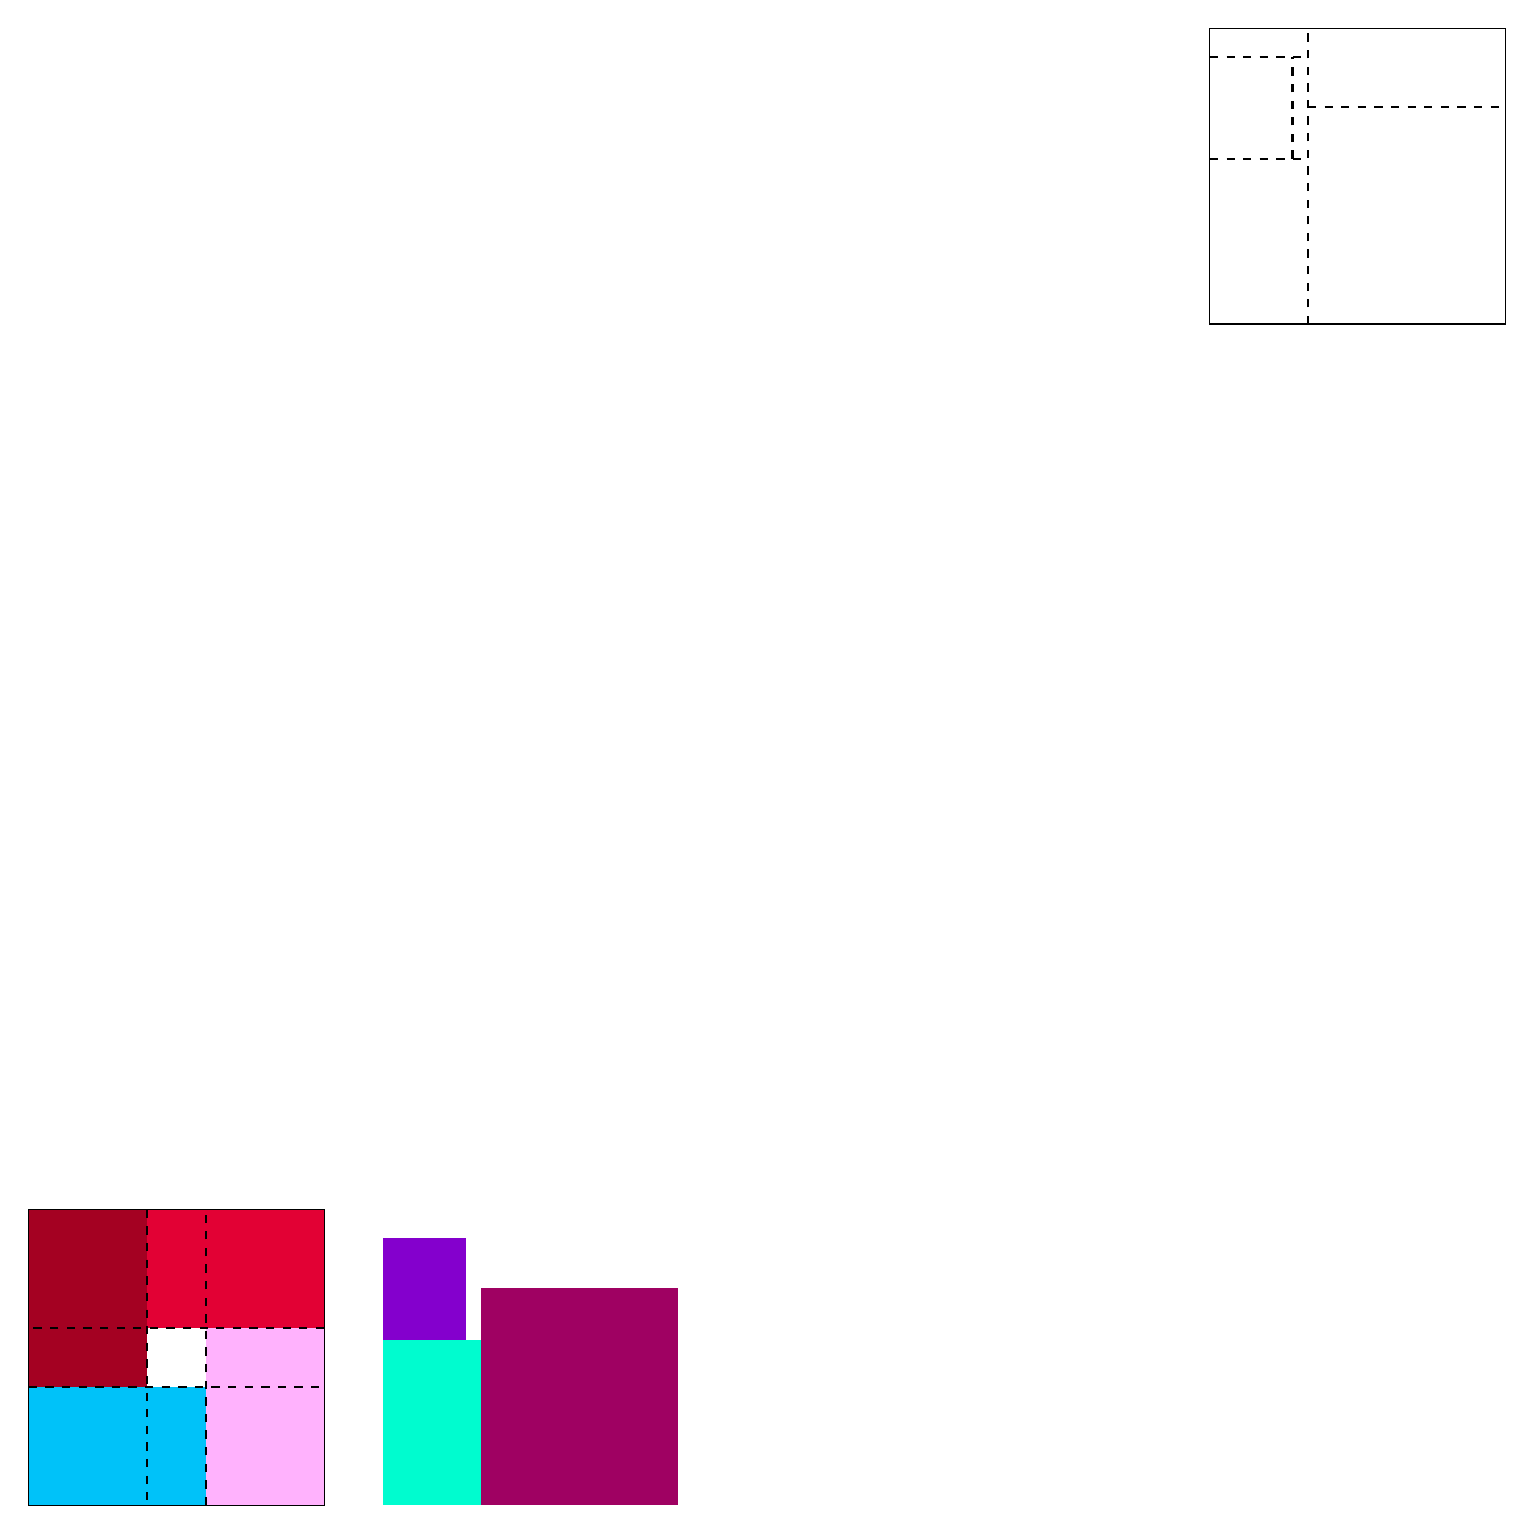
\begin{tikzpicture}[scale=15]

\fill[capri] (0, 0) rectangle +(0.150, 0.100);
\fill[plum] (0.150, 0) rectangle +(0.100, 0.150);
\fill[carmine] (0, 0.100) rectangle +(0.100, 0.150);
\fill[crimson] (0.100, 0.150) rectangle +(0.150, 0.100);
\draw[black] (0,0) rectangle +(0.250, 0.250);
\onslide<2>{\draw[dashed, thick, black] (0,0.100) -- (0.250, 0.100);}
\onslide<3>{\draw[dashed, thick, black] (0.150,0) -- (0.150, 0.250);}
\onslide<4>{\draw[dashed, thick, black] (0.250, 0.150) -- (0.,0.150);}
\onslide<5>{\draw[dashed, thick, black] (0.100,0.250) -- (0.100, 0.0);}

\fill[aquamarine] (0.300,0) rectangle +(0.083, 0.140);
\fill[french] (0.300,0.140) rectangle +(0.070, 0.086);
\fill[jam] (0.383,0) rectangle +(0.167, 0.184);
\draw[black] ++(\kx, \ky) +(0,0) rectangle +(0.250, 0.250);
\onslide<2->{\draw[dashed, thick, black] ++(\kx, \ky) +(0.083,0) -- +(0.083, 0.250);}
\onslide<3->{\draw[dashed, thick, black] ++(\kx, \ky) +(0,0.140) -- +(0.083, 0.140);}
\onslide<4->{\draw[dashed, thick, black] ++(\kx, \ky) +(0,0.226) -- +(0.083, 0.226);}
\onslide<5->{\draw[dashed, thick, black] ++(\kx, \ky) +(0.070,0.140) -- +(0.070, 0.226);}
\onslide<6>{\draw[dashed, thick, black] ++(\kx, \ky) +(0.083,0.184) -- +(0.250, 0.184);}
\end{tikzpicture}
}

\frame{\frametitle{Orthogonal Cuts and Non-Orthogonal (Irregular) Cuts}
\center
``\emph{Orthogonal cuts} are always parallel to one side of a plate (and perpendicular to the other).''

\center
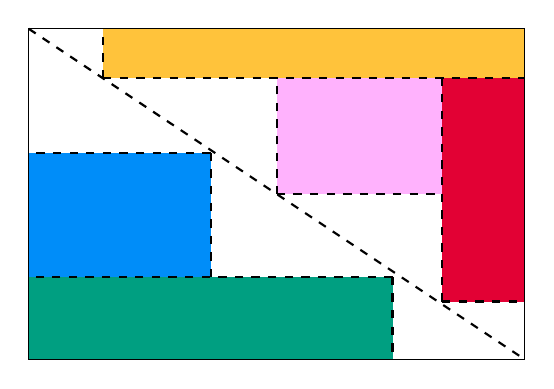
\begin{tikzpicture}[scale=21]

\fill[creepers] (0,0) rectangle +(0.220, 0.050);
\fill[dodger] (0,0.050) rectangle +(0.110, 0.075);
\fill[spark] (0.045,0.170) rectangle +(0.255, 0.030);
\fill[crimson] (0.250,0.035) rectangle +(0.050, 0.135);
\fill[plum] (0.150, 0.100) rectangle +(0.100, 0.070);

\onslide<2->{\draw[dashed, thick, black] (0,0.200) -- (0.300, 0);} % diagonal

\onslide<3->{\draw[dashed, thick, black] (0.045,0.170) -- +(0, 0.030);} % before spark
\onslide<4->{\draw[dashed, thick, black] (0.045,0.170) -- +(0.255, 0.0);} % below spark

\onslide<5->{\draw[dashed, thick, black] (0.250,0.035) -- +(0, 0.135);} % before crimson
\onslide<6->{\draw[dashed, thick, black] (0.250,0.035) -- +(0.050, 0);} % below crimson

\onslide<7->{\draw[dashed, thick, black] (0.150,0.100) -- +(0, 0.070);} % before plum
\onslide<8->{\draw[dashed, thick, black] (0.150,0.100) -- +(0.100, 0);} % below plum

\onslide<9->{\draw[dashed, thick, black] (0.220,0.050) -- (0, 0.050);} % above creepers
\onslide<10->{\draw[dashed, thick, black] (0.220,0.050) -- (0.220, 0);} % after creepers

\onslide<11->{\draw[dashed, thick, black] (0.110,0.125) -- (0, 0.125);} % above dogder
\onslide<12->{\draw[dashed, thick, black] (0.110,0.125) -- (0.110, 0.050);} % after dodger

\draw[black] (0,0) rectangle +(0.300, 0.200);

\end{tikzpicture}
}

\frame{\frametitle{Unrestricted Cuts}
\center
\small``The position of a cut does not need to match a single piece dimension.''

\center
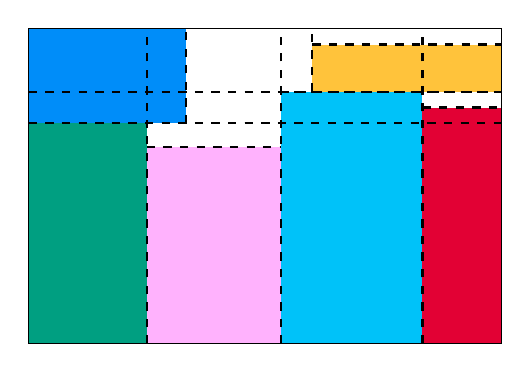
\begin{tikzpicture}[scale=20]

\fill[creepers] (0,0) rectangle +(0.075, 0.140);
\fill[plum] (0.075,0) rectangle +(0.085, 0.125);

\fill[capri] (0.160,0) rectangle +(0.090, 0.160);
\fill[crimson] (0.250,0) rectangle +(0.050, 0.150);

\fill[dodger] (0,0.140) rectangle +(0.100, 0.060);
\fill[spark] (0.180,0.160) rectangle +(0.120, 0.030);

\onslide<2>{\draw[dashed, thick, black] (0.075,0) -- (0.075, 0.200);}
\onslide<3>{\draw[dashed, thick, black] (0.250,0) -- (0.250, 0.200);}
\onslide<4>{\draw[dashed, thick, black] (0,0.140) -- (0.300, 0.140);}
\onslide<5>{\draw[dashed, thick, black] (0,0.160) -- (0.300, 0.160);}

\onslide<6->{\draw[dashed, thick, black] (0.160,0) -- (0.160, 0.200);} % first cut (between plum and capri)
\onslide<7->{\draw[dashed, thick, black] (0,0.140) -- (0.160, 0.140);} % between creepers and dodger
\onslide<8->{\draw[dashed, thick, black] (0.100,0.140) -- (0.100, 0.200);} % after dodger
\onslide<9->{\draw[dashed, thick, black] (0.075,0.125) -- (0.160, 0.125);} % above plum
\onslide<10->{\draw[dashed, thick, black] (0.075,0) -- (0.075, 0.140);} % between creepers and plum
\onslide<11->{\draw[dashed, thick, black] (0.160,0.160) -- (0.300, 0.160);} % below spark
\onslide<12->{\draw[dashed, thick, black] (0.250,0.0) -- (0.250, 0.160);} % between capri and crimson
\onslide<13->{\draw[dashed, thick, black] (0.250,0.150) -- (0.300, 0.150);} % above crimson
\onslide<14->{\draw[dashed, thick, black] (0.180,0.160) -- (0.180, 0.200);} % before spark
\onslide<15->{\draw[dashed, thick, black] (0.180,0.190) -- (0.300, 0.190);} % below spark

\draw[black] (0,0) rectangle +(0.300, 0.200);
\end{tikzpicture}
}

\frame{\frametitle{Constrained Demand}
\center
``There is a limit on the number of copies a piece may be sold.''

\def\kx{0.350}
\def\ky{0}
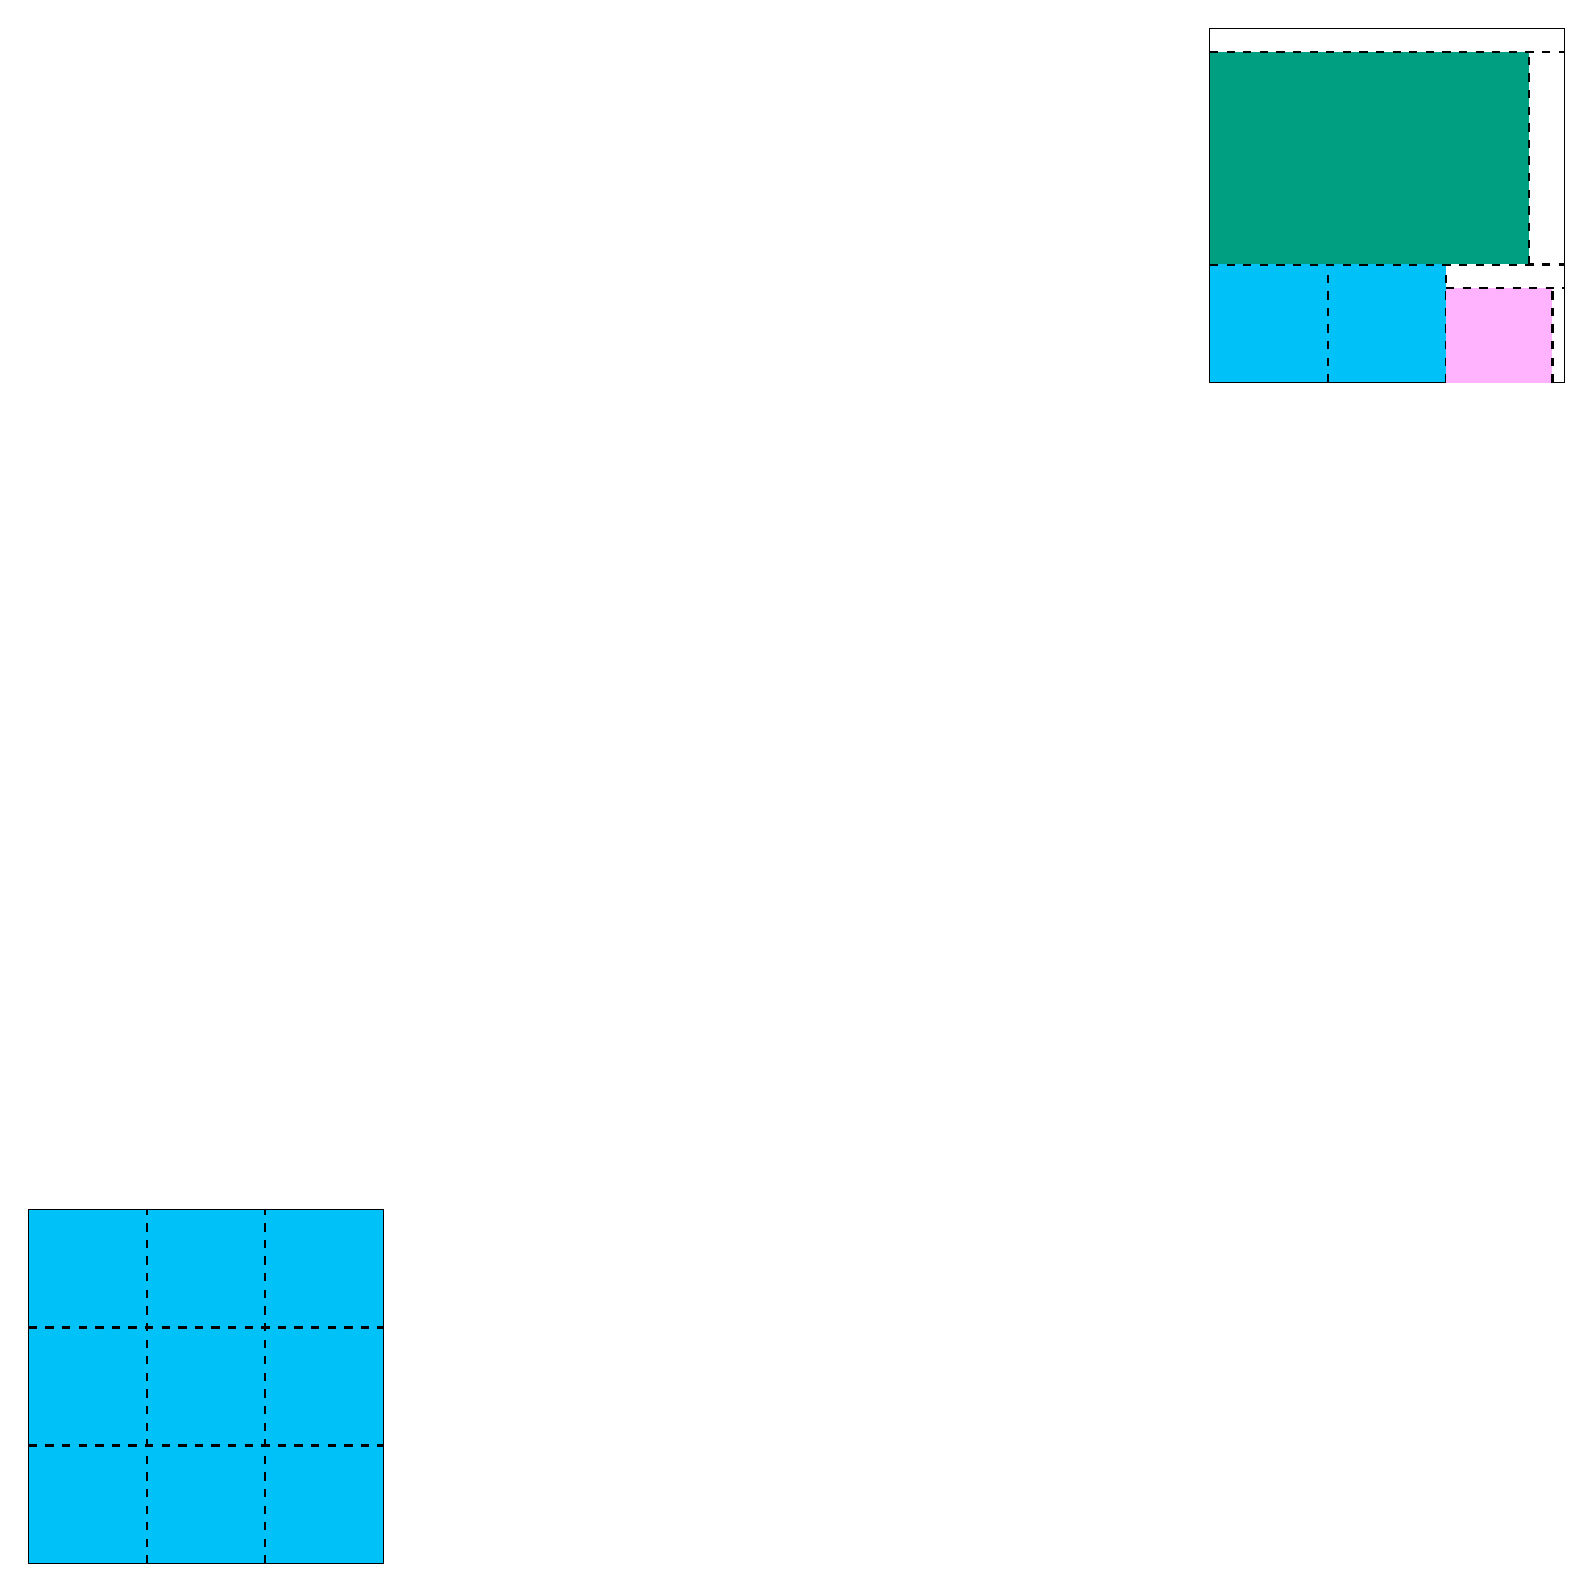
\begin{tikzpicture}[scale=15]
% First Plate
\fill[capri] (0, 0) rectangle +(0.300, 0.300);
\draw[black] (0,0) rectangle +(0.300, 0.300);
\draw[dashed, thick, black] (0,0.100) -- (0.300, 0.100);
\draw[dashed, thick, black] (0,0.200) -- (0.300, 0.200);
\draw[dashed, thick, black] (0.100,0) -- (0.100, 0.300);
\draw[dashed, thick, black] (0.200,0) -- (0.200, 0.300);

% Second Plate
\fill[capri] ++(\kx, \ky) +(0, 0) rectangle +(0.200, 0.100);
\draw[black] ++(\kx, \ky) +(0,0) rectangle +(0.300, 0.300);
\draw[dashed, thick, black] ++(\kx, \ky) +(0,0.100) -- +(0.300, 0.100);
\draw[dashed, thick, black] ++(\kx, \ky) +(0.100,0) -- +(0.100, 0.100);
\draw[dashed, thick, black] ++(\kx, \ky) +(0.200,0) -- +(0.200, 0.100);

\fill[creepers] (\kx, \ky) ++(0, 0.100) rectangle +(0.270, 0.180);
\fill[plum] (\kx, \ky) ++(0.200, 0) rectangle +(0.090, 0.080);

\draw[dashed, thick, black] ++(\kx, \ky) +(0,0.280) -- +(0.300, 0.280);
\draw[dashed, thick, black] ++(\kx, \ky) +(0.270,0.100) -- +(0.270, 0.280);

\draw[dashed, thick, black] ++(\kx, \ky) +(0.200,0.080) -- +(0.300, 0.080);
\draw[dashed, thick, black] ++(\kx, \ky) +(0.290,0) -- +(0.290, 0.080);

\end{tikzpicture}
}

\frame{\frametitle{\(k\)-staged}
\center

{``In the exact \(k\)-staged G2KP, the guillotine is switched at most \(k-1\) times.''}

\def\kx{0}
\def\ky{0}

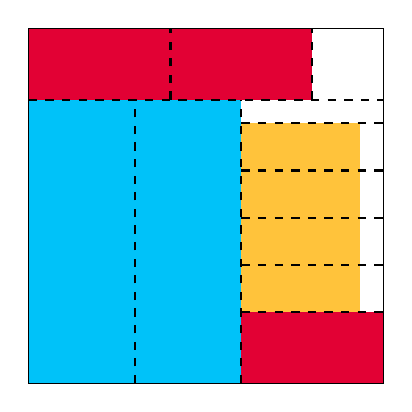
\begin{tikzpicture}[scale=15]

\onslide<3->{\fill[capri] (\kx, \ky) ++(0, 0) rectangle +(0.180, 0.240);}
\onslide<3->{\fill[crimson] (\kx, \ky) ++(0, 0.240) rectangle +(0.240, 0.060);}
\onslide<4->{\fill[crimson] (\kx, \ky) ++(0.180, 0) rectangle +(0.120, 0.060);}
\onslide<6->{\fill[spark] (\kx, \ky) ++(0.180, 0.060) rectangle +(0.100, 0.160);}
\draw[black] (\kx, \ky) ++(0,0) rectangle +(0.300, 0.300);

\onslide<2->{\draw[dashed, thick, black] ++(\kx, \ky) +(0,0.240) -- +(0.300, 0.240);} % first cut

\onslide<3->{\draw[dashed, thick, black] ++(\kx, \ky) +(0.120,0.240) -- +(0.120, 0.300);} % vertical top cuts
\onslide<3->{\draw[dashed, thick, black] ++(\kx, \ky) +(0.240,0.240) -- +(0.240, 0.300);} % vertical top cuts
\onslide<3->{\draw[dashed, thick, black] ++(\kx, \ky) +(0.090,0) -- +(0.090, 0.240);} % vertical bottom cuts
\onslide<3->{\draw[dashed, thick, black] ++(\kx, \ky) +(0.180,0) -- +(0.180, 0.240);} % vertical bottom cuts

\onslide<5->{\draw[dashed, thick, black] ++(\kx, \ky) +(0.180,0.060) -- +(0.300, 0.060);} % third stage cuts
\onslide<6->{\draw[dashed, thick, black] ++(\kx, \ky) +(0.180,0.100) -- +(0.300, 0.100);} % third stage cuts
\onslide<6->{\draw[dashed, thick, black] ++(\kx, \ky) +(0.180,0.140) -- +(0.300, 0.140);} % third stage cuts
\onslide<6->{\draw[dashed, thick, black] ++(\kx, \ky) +(0.180,0.180) -- +(0.300, 0.180);} % third stage cuts
\onslide<6->{\draw[dashed, thick, black] ++(\kx, \ky) +(0.180,0.220) -- +(0.300, 0.220);} % third stage cuts

\end{tikzpicture}

\onslide<4->{\small ``The non-exact \(k\)-staged G2KP adds one extra stage in which the only cuts allowed are the ones that trim plates to the size of pieces''}
}

\frame{\frametitle{No Rotation}
\center
``we never switch length and width during the cutting process''

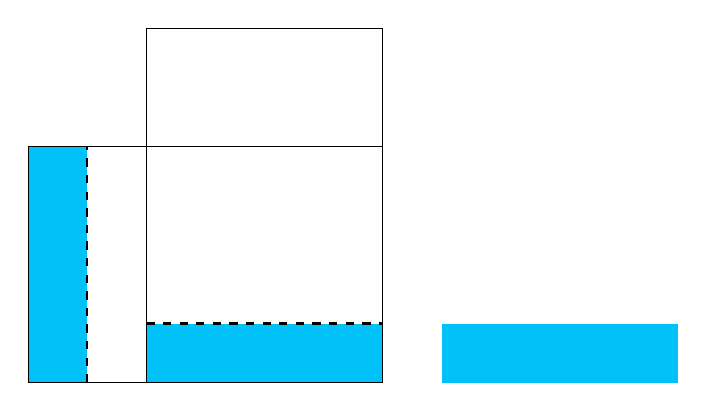
\begin{tikzpicture}[scale=15]

\fill[capri] (0.350, 0) rectangle +(0.200, 0.050); % piece out

\onslide<2>{\fill[capri] (0, 0) rectangle +(0.050, 0.200);} % piece in (first)
\onslide<2>{\draw[dashed, thick, black]  (0.050,0) -- (0.050, 0.200);} % cut (first)
\onslide<1-2>{\draw[black] (0,0) rectangle +(0.300, 0.200);} % plate (first)

\onslide<3>{\fill[capri] (0.100, 0) rectangle +(0.200, 0.050);} % piece in (second)
\onslide<3>{\draw[dashed, thick, black] (0.100,0.050) -- (0.300, 0.050);} % cut (second)
\onslide<3>{\draw[black] (0.100,0) rectangle +(0.200, 0.300);} % plate (second)

\end{tikzpicture}
}

\frame{\frametitle{Summary of the problem characteristics}
\begin{itemize}
\item Knapsack -- maximises profit, single plate.
\item Guillotine Cuts -- from a side to another.
\item Orthogonal Cuts -- only cuts parallel to the sides.
\item Unrestricted Cuts -- may cut in any position.
\item Constrained Demand -- upper bound for pieces in solution.
\item Unlimited Stages -- no limit on cut orientation changes.
\item No rotation -- of pieces or plates.
\end{itemize}
}

\mysection{Prior Work}
\subsection{Seminal Works and Surveys}
\begin{frame}[t]{Seminal Works and Surveys}
\setbeamercovered{transparent=50}
\begin{description}
% gg:65 (first version of unconstrained weakly NP-Hard)
% herz:72 (unconstrained seminal work, introduces cut enumeration)
% cw7 (constrained exact seminal work, introduces cut enumeration)
% iori:2020
% russo:2020
\item<1-1>[1965] Introduces the unconstrained (weakly NP-Hard) G2KP and other variants (no experiments). \alt<1-1>{\alert{\cite{gg:1965}}}{\cite{gg:1965}}
\item<2-2>[1972] Seminal work on the unconstrained G2KP. Introduces `canonical dissecations' (used pervasively).\alt<2-2>{\alert{\cite{herz:1972}}}{\cite{herz:1972}}
\item<3-3>[1977] Seminal work on the constrained G2KP. Treats some symmetries. Proposes classical instances.\alt<3-3>{\alert{\cite{cw:1977}}}{\cite{cw:1977}}
\item<4-4>[2020] Surveys exact methods and relaxations on 2D cutting and packing. \alt<4-4>{\alert{\cite{iori:2020}}}{\cite{iori:2020}}
\item<5-5>[2020] Surveys exact methods and relaxations the G2KP specifically; points out mistakes in the literature. \alt<5-5>{\alert{\cite{russo:2020}}}{\cite{russo:2020}}
\end{description}
\only<1-1>{\alert{\cite{gg:1965}} Gilmore, P. C.; Gomory, R. E. Multistage Cutting Stock Problems of Two and More Dimensions. 10.1287/opre.13.1.94}
\only<2-2>{\alert{\cite{herz:1972}} Herz, J. C. Recursive Computational Procedure for Two-Dimensional Stock Cutting. 10.1147/rd.165.0462}
\only<3-3>{\alert{\cite{cw:1977}} Christofides, N.; Whitlock, C. An Algorithm for Two-Dimensional Cutting Problems. 10.1287/opre.25.1.30}
\only<4-4>{\alert{\cite{iori:2020}} Iori, M.; de Lima, V. L.; Martello, S.; Miyazawa, F. K.; Monaci, M. Exact Solution Techniques for Two-Dimensional Cutting and Packing. 10.1016/j.ejor.2020.06.050}
\only<5-5>{\alert{\cite{russo:2020}} Russo, M.; Boccia, M.; Sforza, A.; Sterle, C. Constrained Two-Dimensional Guillotine Cutting Problem: Upper-Bound Review and Categorization. 10.1111/itor.12687}
\end{frame}

\subsection{Formulations}
\begin{frame}{Formulations}
\setbeamercovered{transparent=50}
\begin{description}
\item<1-1>[2008] The first MILP formulation for unlimited stages. Mostly of theoretical interest. \alt<1-1>{\alert{\cite{messaoud:2008}}}{\cite{messaoud:2008}}
\item<2-2>[2010] Two- and (restricted) three-staged formulations for the G2CSP. Not the first \(k\)-staged formulation. \alt<2-2>{\alert{\cite{silva:2010}}}{\cite{silva:2010}}
\item<3-3>[2013] Compares three two-staged MILP formulations including the work mentioned above.\alt<3-3>{\alert{\cite{furini:2013}}}{\cite{furini:2013}}
\item<4-4>[2016] The first MILP formulation for the unlimited stages G2KP able to solve medium-sized intances.\alt<4-4>{\alert{\cite{furini:2016}}}{\cite{furini:2016}}
\item<5-5>[2020] Three new competitive formulations were proposed recently.\alt<5-5>{\alert{\cite{martin:2020:models}}}{\cite{martin:2020:models}}
\end{description}
\only<1-1>{\alert{\cite{messaoud:2008}} Ben Messaoud, S.; Chu, C.; Espinouse, M.-L. Characterization and Modelling of Guillotine Constraints. 10.1016/j.ejor.2007.08.029 }
\only<2-2>{\alert{\cite{silva:2010}} Silva, E.; Alvelos, F.; Valério de Carvalho, J. M. An Integer Programming Model for Two- and Three-Stage Two-Dimensional Cutting Stock Problems. 10.1016/j.ejor.2010.01.039 }
\only<3-3>{\alert{\cite{furini:2013}} Furini, F.; Malaguti, E. Models for the Two-Dimensional Two-Stage Cutting Stock Problem with Multiple Stock Size. 10.1016/j.cor.2013.02.026}
\only<4-4>{\alert{\cite{furini:2016}} Furini, F.; Malaguti, E.; Thomopulos, D. Modeling Two-Dimensional Guillotine Cutting Problems via Integer Programming. 10.1287/ijoc.2016.0710}
\only<5-5>{\alert{\cite{martin:2020:models}} Martin, M.; Morabito, R.; Munari, P. A Top-down Cutting Approach for Modeling the Constrained Two- and Three-Dimensional Guillotine Cutting Problems. 10.1080/01605682.2020.1813640.}

\end{frame}

\begin{frame}[fragile]
\frametitle{Current Work}
\centering
\begin{description}
%\item[(this thesis)] Old algorithms are implemented and tested. The influence of the datasets in the comparisons becomes apparent.
\item[(this work)] \begin{itemize}
\item enhances of a state-of-the-art formulation by cutting down model size and symmetries;
\item adaptation of a previous reduction to our context also reducing model size and symmtries;
\item new results for recently proposed and more challenging instances;
\end{itemize}
\end{description}
\end{frame}

\mysection{Reductions}
\subsection{Discretization}
\frame{\frametitle{Discretization}
\center
We can restrict cuts to linear combinations of piece dimensions (constrained by their demand) without losing optimality.

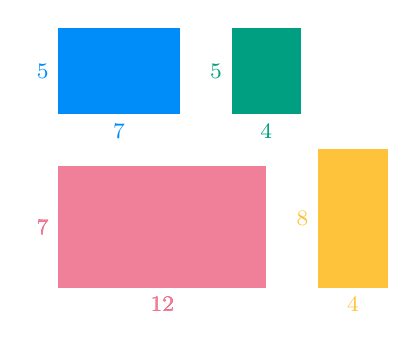
\begin{tikzpicture}[scale=22]
\fill[creepers] (0.10,0.10) rectangle +(0.04, 0.05);
\node[creepers] at (0.12, 0.10) [below]{\dslidefs 4};
\node[creepers] at (0.10, 0.125) [left]{\dslidefs 5};
\fill[dodger] (0,0.10) rectangle +(0.07, 0.05);
\node[dodger] at (0.035, 0.10) [below]{\dslidefs 7};
\node[dodger] at (0, 0.125) [left]{\dslidefs 5};
\fill[spark] (0.15,0) rectangle +(0.04, 0.08);
\node[spark] at (0.17, 0) [below]{\dslidefs 4};
\node[spark] at (0.15, 0.04) [left]{\dslidefs 8};
\onslide<-3>{
	\fill[crimson] (0,0) rectangle +(0.12, 0.07);
	\node[crimson] at (0.06, 0) [below]{\dslidefs 12};
	\node[crimson] at (0, 0.035) [left]{\dslidefs 7};
}
\onslide<4->{
	\fill[crimson!50] (0,0) rectangle +(0.12, 0.07);
	\node[crimson!50] at (0.06, 0) [below]{\dslidefs 12};
	\node[crimson!50] at (0, 0.035) [left]{\dslidefs 7};
}
\end{tikzpicture}
\hspace{0.25cm} % ----------------------------------------------------
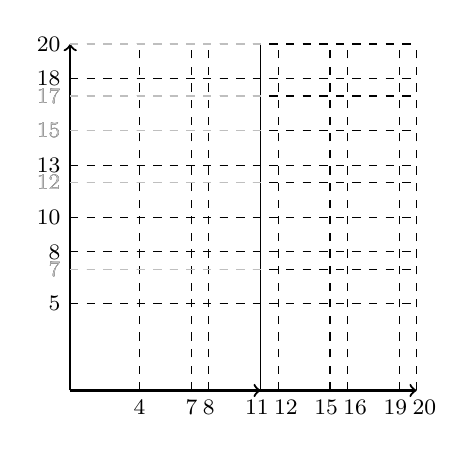
\begin{tikzpicture}[scale=22]
\draw[thick,->] (0, 0) -- (0,0.20); % y axis
\onslide<-2>{\draw[thick,->] (0, 0) -- (0.20,0);} % x axis
\onslide<3->{\draw[thick,->] (0, 0) -- (0.11,0);} % x axis

%left: 5, 7, 8, 10, 12, 13, 15, 17, 18, 20
\node at (0, 0.05) [left]{\dslidefs 5};
\onslide<-4>{\node at (0, 0.07) [left]{\dslidefs 7};}
\node at (0, 0.08) [left]{\dslidefs 8};
\node at (0, 0.10) [left]{\dslidefs 10};
\onslide<-4>{\node at (0, 0.12) [left]{\dslidefs 12};}
\node at (0, 0.13) [left]{\dslidefs 13};
\onslide<-4>{\node at (0, 0.15) [left]{\dslidefs 15};}
\onslide<-4>{\node at (0, 0.17) [left]{\dslidefs 17};}
\node at (0, 0.18) [left]{\dslidefs 18};
\node at (0, 0.20) [left]{\dslidefs 20};
\onslide<5>{\node[black!25] at (0, 0.07) [left]{\dslidefs 7};}
\onslide<5>{\node[black!25] at (0, 0.12) [left]{\dslidefs 12};}
\onslide<5>{\node[black!25] at (0, 0.15) [left]{\dslidefs 15};}
\onslide<5>{\node[black!25] at (0, 0.17) [left]{\dslidefs 17};}

% horizontal
\onslide<-2>{
	\draw[dashed, black] (0,0.05) -- (0.2, 0.05);
	\draw[dashed, black] (0,0.07) -- (0.2, 0.07);
	\draw[dashed, black] (0,0.08) -- (0.2, 0.08);
	\draw[dashed, black] (0,0.10) -- (0.2, 0.10);
	\draw[dashed, black] (0,0.12) -- (0.2, 0.12);
	\draw[dashed, black] (0,0.13) -- (0.2, 0.13);
	\draw[dashed, black] (0,0.15) -- (0.2, 0.15);
	\draw[dashed, black] (0,0.17) -- (0.2, 0.17);
	\draw[dashed, black] (0,0.18) -- (0.2, 0.18);
	\draw[dashed, black] (0,0.20) -- (0.2, 0.20);
}
\onslide<3->{
	\draw[dashed, black] (0,0.05) -- (0.11, 0.05);
	\draw[dashed, black] (0,0.07) -- (0.11, 0.07);
	\draw[dashed, black] (0,0.08) -- (0.11, 0.08);
	\draw[dashed, black] (0,0.10) -- (0.11, 0.10);
	\draw[dashed, black] (0,0.12) -- (0.11, 0.12);
	\draw[dashed, black] (0,0.13) -- (0.11, 0.13);
	\draw[dashed, black] (0,0.15) -- (0.11, 0.15);
	\draw[dashed, black] (0,0.17) -- (0.11, 0.17);
	\draw[dashed, black] (0,0.18) -- (0.11, 0.18);
	\draw[dashed, black] (0,0.20) -- (0.11, 0.20);
}

% below: 4, 7, 8, 11, 12, 15, 16, 19, 20
\node at (0.04, 0) [below]{\dslidefs 4};
\node at (0.07, 0) [below]{\dslidefs 7};
\node at (0.08, 0) [below]{\dslidefs 8};
\node at (0.11, 0) [below]{\dslidefs {11~~}};
\onslide<-2>{
\node at (0.12, 0) [below]{\dslidefs {~~12}};
\node at (0.15, 0) [below]{\dslidefs {15~~}};
\node at (0.16, 0) [below]{\dslidefs {~~16}};
\node at (0.19, 0) [below]{\dslidefs {19~~}};
\node at (0.20, 0) [below]{\dslidefs {~~20}};
}

% vertical
\draw[dashed, black] (0.04,0) -- (0.04, 0.2);
\draw[dashed, black] (0.07,0) -- (0.07, 0.2);
\draw[dashed, black] (0.08,0) -- (0.08, 0.2);
\draw[dashed, black] (0.11,0) -- (0.11, 0.2);
\onslide<-2>{
	\draw[dashed, black] (0.12,0) -- (0.12, 0.2);
	\draw[dashed, black] (0.15,0) -- (0.15, 0.2);
	\draw[dashed, black] (0.16,0) -- (0.16, 0.2);
	\draw[dashed, black] (0.19,0) -- (0.19, 0.2);
	\draw[dashed, black] (0.20,0) -- (0.20, 0.2);
}

\onslide<2>{\draw (0.11,0) -- (0.11, 0.2);}

\onslide<5>{
	\draw[dashed, black!25] (0,0.07) -- (0.11, 0.07);
	\draw[dashed, black!25] (0,0.12) -- (0.11, 0.12);
	\draw[dashed, black!25] (0,0.15) -- (0.11, 0.15);
	\draw[dashed, black!25] (0,0.17) -- (0.11, 0.17);
	\draw[dashed, black!25] (0,0.20) -- (0.11, 0.20);
}

\end{tikzpicture}
}

\subsection{Plate-Size Normalization}
\frame{\frametitle{Plate-Size Normalization}
\center
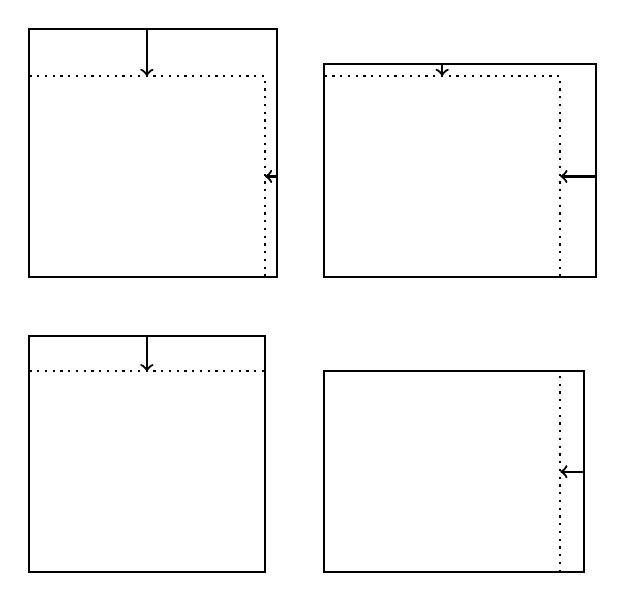
\begin{tikzpicture}[scale=15]
\draw[dotted, thick] (0, 0) rectangle +(0.20, 0.17);
\draw[black, thick] (0, 0) rectangle +(0.20, 0.20);
\draw[thick,->] (0.1, 0.20) -- (0.1,0.17);

\draw[dotted, thick] (0.25, 0) rectangle +(0.20, 0.17);
\draw[black, thick] (0.25, 0) rectangle +(0.22, 0.17);
\draw[thick,->] (0.47, 0.085) -- (0.45,0.085);

\draw[dotted, thick] (0, 0.25) rectangle +(0.20, 0.17);
\draw[black, thick] (0, 0.25) rectangle +(0.21, 0.21);
\draw[thick,->] (0.1, 0.46) -- (0.1,0.42);
\draw[thick,->] (0.21, 0.335) -- (0.20,0.335);

\draw[dotted, thick] (0.25, 0.25) rectangle +(0.20, 0.17);
\draw[black, thick] (0.25, 0.25) rectangle +(0.23, 0.18);
\draw[thick,->] (0.35, 0.43) -- (0.35,0.42);
\draw[thick,->] (0.48, 0.335) -- (0.45,0.335);

\end{tikzpicture}
}

% TODO: check if it is worth putting here a slide about other discretizations

\subsection{Previous Reductions}
\frame{\frametitle{Previous Reductions}
\begin{itemize}
%\item[(this thesis)] Old algorithms are implemented and tested. The influence of the datasets in the comparisons becomes apparent.
\item Redundant-Cut
\begin{itemize}
\item Remove trim cuts if alternative cut patterns exist.
\item Does not affect the number of plates (constraints).
\item Is superseeded by our enhanced formulation.
\end{itemize}
\item Cut-Position
\begin{itemize}
\item Removes unrestricted cuts from small plates.
\item If 6 pieces do not fit, there is no loss.
\item Affects both number of variables and constraints.
\end{itemize}
\end{itemize}
% start with the one that links to the piece extraction symmetries
% "It is not a problem we had a proble reimplementing it because our enhanced model makes it obsolete."
% what is redundant-cut and cut position
}

\frame{\frametitle{Unrestricted Cuts (Revisited)}
\center
\small``The position of a cut does not need to match a single piece dimension.''

\center
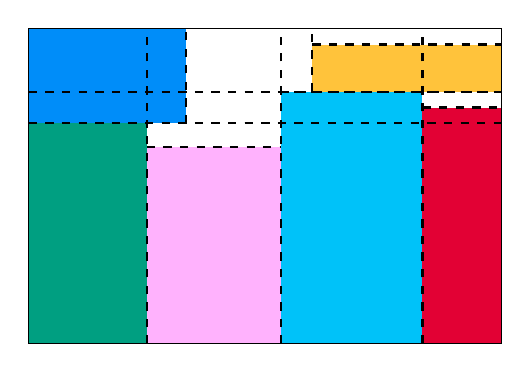
\begin{tikzpicture}[scale=20]

\fill[creepers] (0,0) rectangle +(0.075, 0.140);
\fill[plum] (0.075,0) rectangle +(0.085, 0.125);

\fill[capri] (0.160,0) rectangle +(0.090, 0.160);
\fill[crimson] (0.250,0) rectangle +(0.050, 0.150);

\fill[dodger] (0,0.140) rectangle +(0.100, 0.060);
\fill[spark] (0.180,0.160) rectangle +(0.120, 0.030);

\onslide<2>{\draw[dashed, thick, black] (0.075,0) -- (0.075, 0.200);}
\onslide<3>{\draw[dashed, thick, black] (0.250,0) -- (0.250, 0.200);}
\onslide<4>{\draw[dashed, thick, black] (0,0.140) -- (0.300, 0.140);}
\onslide<5>{\draw[dashed, thick, black] (0,0.160) -- (0.300, 0.160);}

\onslide<6->{\draw[dashed, thick, black] (0.160,0) -- (0.160, 0.200);} % first cut (between plum and capri)
\onslide<7->{\draw[dashed, thick, black] (0,0.140) -- (0.160, 0.140);} % between creepers and dodger
\onslide<8->{\draw[dashed, thick, black] (0.100,0.140) -- (0.100, 0.200);} % after dodger
\onslide<9->{\draw[dashed, thick, black] (0.075,0.125) -- (0.160, 0.125);} % above plum
\onslide<10->{\draw[dashed, thick, black] (0.075,0) -- (0.075, 0.140);} % between creepers and plum
\onslide<11->{\draw[dashed, thick, black] (0.160,0.160) -- (0.300, 0.160);} % below spark
\onslide<12->{\draw[dashed, thick, black] (0.250,0.0) -- (0.250, 0.160);} % between capri and crimson
\onslide<13->{\draw[dashed, thick, black] (0.250,0.150) -- (0.300, 0.150);} % above crimson
\onslide<14->{\draw[dashed, thick, black] (0.180,0.160) -- (0.180, 0.200);} % before spark
\onslide<15->{\draw[dashed, thick, black] (0.180,0.190) -- (0.300, 0.190);} % below spark

\draw[black] (0,0) rectangle +(0.300, 0.200);
\end{tikzpicture}
}
% repeat frame about restricted here

%\frame{\frametitle{Furini's Model}
%}
\mysection{Formulations}

\subsection{Our Formulation}
\frame{\frametitle{Our Formulation}
\begin{align*}
\bm{max.} & \sum_{\textcolor{crimson}{(i, j) \in E}} p_i \textcolor{crimson}{e_{ij}}\\
\bm{s.t.} & \specialcell{\textcolor{crimson}{\sum_{j \in E_{i*}} e_{ij}} \leq u_i \hspace*{\fill} \forall i \in \bar{J},}\\
          & \specialcell{\sum_{o \in O}\sum_{q \in Q_{0o}} x^o_{q0} + \sum_{i \textcolor{crimson}{\in E_{*0}}} \textcolor{crimson}{e_{i0}} \leq 1 \hspace*{\fill},}\\
          & \specialcell{\sum_{o \in O}\sum_{q \in Q_{jo}} x^o_{qj} + \sum_{i \textcolor{crimson}{\in E_{*j}}} \textcolor{crimson}{e_{ij}} \leq \sum_{k \in J}\sum_{o \in O}\sum_{q \in Q_{ko}} a^o_{qkj} x^o_{qk} \hspace*{0.05\textwidth} \forall j \in J, j \neq 0,}\\
\end{align*}
}

\subsection{Furini's Formulation}
\frame{\frametitle{Furini's Formulation}
\begin{align*}
\bm{max.} & \sum_{j \textcolor{creepers}{\in \bar{J}}} p_j \textcolor{creepers}{y_j}\\
% UNFORTUNATELY, THE HSPACE BELOW MAY NEED MANUAL ADJUSTMENT
\bm{s.t.} & \specialcell{\textcolor{creepers}{y_j} \leq u_j \hspace*{\fill} \forall j \in \bar{J},}\\
	    & \specialcell{\sum_{o \in O}\sum_{q \in Q_{0o}} x^o_{q0} + \textcolor{creepers}{y_0} \leq 1 \hspace*{\fill} ,}\\
            & \specialcell{\sum_{o \in O}\sum_{q \in Q_{jo}} x^o_{qj} + \textcolor{creepers}{y_j} \leq \sum_{k \in J}\sum_{o \in O}\sum_{q \in Q_{ko}} a^o_{qkj} x^o_{qk} \hspace*{0.15\textwidth} \forall j \in \bar{J}, j \neq 0,}\\
            & \specialcell{\textcolor{creepers}{\sum_{o \in O}\sum_{q \in Q_{jo}} x^o_{qj} \leq \sum_{k \in J}\sum_{o \in O}\sum_{q \in Q_{ko}} a^o_{qkj} x^o_{qk} \hspace*{\fill} \forall j \in J\setminus\bar{J},}}\\
\end{align*}
}
% REPEAT THE REDUCE PLATE-SIZE MODEL HERE? Says this is why the
% redundant-cut becomes obsolete.

%\frame{\frametitle{Pricing}
% Write this damned pseudo-code
%}

\mysection{Experimental Results}
\frame{\frametitle{The three data sources}

There is data from three data sources in the experiments:
\begin{description}
\item[\textcolor{creepers}{Original}] Data from~\cite{furini:2016,thomopulos:2016}.
\begin{itemize}
\item Other machine and solver (CPLEX).
\item Unspecified implementation language.
\item Implementation was not available.
\end{itemize}
\item[\textcolor{dodger}{Faithful}] Our reimplementation of \textcolor{creepers}{original}.
\begin{itemize}
\item Uses Julia, JuMP, and Gurobi.
\item Matches number of variables and constraints closely.
\end{itemize}
\item[\textcolor{crimson}{Enhanced}] Our enhanced formulation based on~\cite{furini:2016,thomopulos:2016}.
\begin{itemize}
\item Compatible with the Cut-Position and the pricing, supersedes Redundant-cut.
\end{itemize}
\end{description}
}

\frame{\frametitle{Comparison of LP algorithms (\textcolor{dodger}{Faithful})}
\center
All numbers are running times in seconds.
\begin{tabular}{@{\extracolsep{4pt}}lrrrrr@{}}
\hline\hline
Instance & \multicolumn{2}{c}{Dual Simplex} & \multicolumn{2}{c}{Barrier} & DS + B \\\cline{2-3}\cline{4-5}
& N. P. & Priced & N. P. & Priced & Priced \\\hline
CU1 & 27.37 & 3.79 & 24.18 & 3040.82 & \textbf{3.58} \\
STS4 & 93.49 & 48.80 & 49.94 & 7851.30 & \textbf{47.75} \\
STS4s & 103.20 & 39.29 & 43.74 & 8470.41 & \textbf{38.36} \\
gcut9 & 226.68 & \textbf{3.92} & 85.77 & 2060.04 & 4.01 \\
okp1 & 51.95 & 38.89 & \textbf{32.41} & -- & 38.79 \\
okp4 & 98.25 & 144.30 & \textbf{72.09} & -- & 141.53 \\
okp5 & 178.13 & 252.09 & \textbf{96.38} & -- & 239.44 \\\hline\hline
\end{tabular}
}

\frame{\frametitle{\textcolor{creepers}{Original} vs \textcolor{dodger}{Faithful}}
\center
The closer to 100.00\% the better.
\Wider{
\begin{tabular}{lcrrrr}
\hline\hline
Variant & N. M. & \textcolor{creepers}{O. \#v} & \textcolor{dodger}{F. \%v} & \textcolor{creepers}{O. \#p} & \textcolor{dodger}{F. \%p}\\\hline
Complete PP-G2KP & 0 & 156M & 100.00 & 1.88M & 100.00\\
Complete +Cut-Position & 0 & 103M & 99.99 & 1.73M & 100.01\\
Complete +Redundant-Cut & 0 & 121M & 109.94 & 1.88M & 100.00\\
PP-G2KP (CP + RC) & 0 & 74M & 120.05 & 1.73M & 100.01\\
Restricted PP-G2KP & 0 & \(\approx\)5M & 99.28 & 0.30M & 99.99\\
Priced Restricted PP-G2KP & 1 & \(\approx\)4M & 102.20 & 0.30M & 99.99\\
(no purge) Priced PP-G2KP & 10 & \(\approx\)15M & 93.74 & 1.64M & 100.01\\
Priced PP-G2KP & 10 & \(\approx\)15M & 31.92 & 1.64M & 25.55\\\hline\hline
\end{tabular}
}%Wider
}

% This disable logo only works if done before the frame.
% Also, it needs to be reenabled after.
\placelogofalse % disable logo because it enters the table
\frame{\frametitle{\textcolor{dodger}{Faithful} vs \textcolor{crimson}{Enhanced} (Model Size)}
\center
Last column has the sum of running times for the instances solved.
\Wider{
\begin{tabular}{lrrrrrr}
\hline\hline
Variant & \#e & \#m & \#s & \#b & \#variables & S. T. \\\hline
\textcolor{dodger}{Faithful} & -- & 59 & 53 & 0 & 88,901,964 & 41,257\\
\textcolor{crimson}{Enhanced} & -- & 59 & 58 & 2 & 3,216,774 & 14,738\\
\textcolor{dodger}{F}. +Normalizing & -- & 59 & 56 & 0 & 60,316,964 & 27,678\\
\textcolor{crimson}{E}. +Normalizing & -- & 59 & 59 & 52 & 2,733,125 & 14,169\\
\textcolor{dodger}{F}. +N. +Warming & -- & 59 & 56 & 0 & 60,316,964 & 28,142\\
\textcolor{crimson}{E}. +N. +Warming & -- & 59 & 59 & 4 & 2,733,125 & 9,778\\
Priced \textcolor{dodger}{F}. +N. +W. & 8 & 50 & 55 & 0 & 3,210,857 & 6,719\\
Priced \textcolor{crimson}{E}. +N. +W. & 8 & 51 & 59 & 1 & 600,778 & 9,108\\
P. \textcolor{dodger}{F}. +N. +W. -Purge & 8 & 50 & 55 & 0 & 8,072,810 & 6,854\\
P. \textcolor{crimson}{E}. +N. +W. -Purge & 8 & 51 & 59 & 0 & 1,021,526 & 9,209\\\hline\hline
\end{tabular}
} % Wider
}

\begin{comment}
\frame{\frametitle{\textcolor{dodger}{Faithful} vs \textcolor{crimson}{Enhanced} (Model Size)}
\Wider{
\begin{tabular}{lrrrrrr}
\hline\hline
Variant & \#e & \#m & \#s & \#b & \#variables & \#plates \\\hline
\textcolor{dodger}{Faithful} & -- & 59 & 53 & 0 & 88,901,964 & 1,738,366 \\
\textcolor{crimson}{Enhanced} & -- & 59 & 58 & 2 & 3,216,774 & 231,836 \\
\textcolor{dodger}{F}. +Normalizing & -- & 59 & 56 & 0 & 60,316,964 & 610,402 \\
\textcolor{crimson}{E}. +Normalizing & -- & 59 & 59 & 52 & 2,733,125 & 145,157 \\
\textcolor{dodger}{F}. +N. +Warming & -- & 59 & 56 & 0 & 60,316,964 & 610,402 \\
\textcolor{crimson}{E}. +N. +Warming & -- & 59 & 59 & 4 & 2,733,125 & 145,157 \\
Priced \textcolor{dodger}{F}. +N. +W. & 8 & 50 & 55 & 0 & 3,210,857 & 174,214 \\
Priced \textcolor{crimson}{E}. +N. +W. & 8 & 51 & 59 & 1 & 600,778 & 64,904 \\
P. \textcolor{dodger}{F}. +N. +W. -Purge & 8 & 50 & 55 & 0 & 8,072,810 & 544,892 \\
P. \textcolor{crimson}{E}. +N. +W. -Purge & 8 & 51 & 59 & 0 & 1,021,526 & 134,102 \\\hline\hline
\end{tabular}
} % Wider

}
\frame{\frametitle{\textcolor{dodger}{Faithful} vs \textcolor{crimson}{Enhanced} (Times)}
\Wider{
\begin{tabular}{lrrrrrr}
\hline\hline
Variant & \#e & \#m & \#s & \#b & T. T. & S. T. T. \\\hline
\textcolor{dodger}{Faithful} & -- & 59 & 53 & 0 & 106,057           & 41,257 \\
\textcolor{crimson}{Enhanced} & -- & 59 & 58 & 2 & 25,538           & 14,738 \\
\textcolor{dodger}{F}. +Normalizing & -- & 59 & 56 & 0 & 60,078     & 27,678 \\
\textcolor{crimson}{E}. +Normalizing & -- & 59 & 59 & 52 & 14,169   & 14,169 \\
\textcolor{dodger}{F}. +N. +Warming & -- & 59 & 56 & 0 & 60,542     & 28,142 \\
\textcolor{crimson}{E}. +N. +Warming & -- & 59 & 59 & 4 & 9,778     & 9,778 \\
Priced \textcolor{dodger}{F}. +N. +W. & 8 & 50 & 55 & 0 & 49,919    & 6,719 \\
Priced \textcolor{crimson}{E}. +N. +W. & 8 & 51 & 59 & 1 & 9,108    & 9,108 \\
P. \textcolor{dodger}{F}. +N. +W. -Purge & 8 & 50 & 55 & 0 & 50,054 & 6,854 \\
P. \textcolor{crimson}{E}. +N. +W. -Purge & 8 & 51 & 59 & 0 & 9,209 & 9,209 \\\hline\hline
\end{tabular}
} % Wider
}
\end{comment}

\frame{\frametitle{Results over harder instances (\textcolor{crimson}{Enhanced})}
\Wider{
\begin{tabular}{lrrrrrrr}
\hline\hline
C. & V. & \#m & Avg. \#v & Avg. \#p & T. T. & \#s & Avg. S. T. \\\hline
\multirow{3}{*}{1} & Not P. & 20 & 1,787,864 & 22,316 & 172,574 & 5 & 2,114.85 \\
                   & R. P. & 13 & 467,692 & 17,139 & 180,051 & 5 & 3,610.29 \\
\vspace{1.5mm}     & P. & 5 & 264,315 & 11,978 & 196,733 & 3 & 4,377.77 \\
\multirow{3}{*}{2} & Not P. & 20 & 1,533,490 & 18,638 & 167,973 & 5 & 1,194.68 \\
                   & R. P. & 20 & 453,159 & 18,638 & 155,184 & 8 & 3,198.11 \\
\vspace{1.5mm}     & P. & 8 & 394,613 & 9,735 & 178,812 & 4 & 1,503.01 \\
\multirow{3}{*}{3} & Not P. & 20 & 2,895,300 & 33,249 & 171,155 & 5 & 1,831.11 \\
                   & R. P. & 10 & 431,913 & 15,895 & 174,569 & 5 & 2,513.80 \\
\vspace{1.5mm}     & P. & 5 & 372,597 & 13,287 & 179,712 & 4 & 1,728.08 \\
\multirow{3}{*}{4} & Not P. & 20 & 3,201,374 & 35,197 & 167,776 & 7 & 3,910.89 \\
                   & R. P. & 10 & 497,802 & 17,011 & 197,047 & 2 & 1,323.65 \\
                   & P. & 2 & 211,093 & 14,227 & 199,477 & 2 & 2,538.79 \\\hline\hline
\end{tabular}
} % Wider
}
% Re-enable the logo.
\placelogotrue % now there are no more tables

\frame{\frametitle{Summary of current results}
\begin{itemize}
\item The choice of LP algorithm is important.
\item Our reimplementation seems reasonably fair.
\item \textcolor{crimson}{Enhanced} takes \(\approx\)4 hours to solve all instances...
\begin{itemize}
\item ...while \textcolor{dodger}{Faithful} takes 12 hours to solve 53 of 59.
\end{itemize}
\item For the new and more challenging instances:
\begin{itemize}
\item 17 new optimal solutions (unrestricted).
\item Better lower bounds for 25 instances.
\item Better upper bounds for 58 instances.
\end{itemize}
\end{itemize}
}

% Future works start

\mysection{Future works}
\frame{\frametitle{Two central tracks}
\begin{description}
\item[Flexibility] \begin{itemize}
\item The primary motivation for using a MILP formulation.
\item Seldomly explored empirically.
\item No interest or absence of positive results?
\end{itemize}
\item[Systematic] \begin{itemize}
\item MILP formulations for unlimited stages are recent.
\item Formulations are adaptable but compared over a single problem.
\item A doctorate thesis has a larger scope.
\end{itemize}
\end{description}
}

\frame{\frametitle{Flexibility (possibilities)}
The possibilities of adaptation include:
\begin{itemize}
\item The Guillotine 2D variant of:
\begin{itemize}
\item Multiple Knapsack Problem (G2MKP)
\item Orthogonal Packing Problem (G2OPP)
\item Strip Packing Problem (G2SPP)
\item Cutting Stock Problem (G2CSP)
\end{itemize}
\item The homogeneous and heterogeneous variants of G2MKP and G2CSP.
\item The rotation variant of G2KP and all problems above.
\end{itemize}
}

\frame{\frametitle{Systematization (possibilities)}
\begin{itemize}
\item Systematically consider all literature instances.
\item Compare with the recent Martin's works.
\item Perhaps compare to other generic solving methods.
\end{itemize}
}

\frame{\frametitle{Other research possibilities}
\begin{description}
\item[VRPSolver] Branch-Cut-and-Price based exact solver for VRP with impressive results for the 1D-BPP.
\item[Matheuristic] How to make the heuristic for MIP-start adaptation-oblivious?
\item[Pricing] Propose a pricing procedure more adequate for our enhanced formulation.
\item[Symmetries] It is clear that the formulation has yet many symmetries.
\end{description}
}

\frame{\frametitle{Plan of action}
\Wider{
\begin{tabular}{@{\extracolsep{-4pt}}lccccccccc@{}}
\hline\hline
Task & Nov & Dec & Jan & Feb & Mar & Apr & May & Jun & Jul \\\hline
Simpler Adaptations & \checkmark & \checkmark & \checkmark & & & & & & \\
Partial Catalogue & & \checkmark & \checkmark & \checkmark & & & & & \\
Preliminar Experiments & & \checkmark & \checkmark & & & & & & \\
Conference Paper & & & \checkmark & \checkmark & \checkmark & & & & \\
Advanced Adaptations & & & & \checkmark & \checkmark & \checkmark & & & \\
Alternative Tracks & & & & \checkmark & \checkmark & \checkmark & & & \\
Final Experiments & & & & & \checkmark & \checkmark & \checkmark & & \\
Thesis Writing & & & & & & & \checkmark & \checkmark & \checkmark \\\hline\hline
\end{tabular}
}%Wider
}

\frame{\frametitle{Changes in the plan}
\begin{itemize}
\item We already submitted a G2CSP short paper to LAGOS 2021.
\begin{itemize}
\item In one day, we adapted the code to the G2CSP.
\item In two weeks, we ran experiments and submitted the short paper.
\item The adaptations are easy now that the `core' is done.
\item We should aim for a full paper in the `Conference paper' slot.
\end{itemize}
\item We are trying to model G2KP (or an easier variant) with VRPSolver.
\begin{itemize}
\item Eduardo Uchoa has shown interest in collaborating.
\end{itemize}
\end{itemize}
}

\bibliographystyle{splncs03.bst}

\backupbegin
\setbeamertemplate{footline}{}
\begin{frame}[allowframebreaks]{References}
\small
\bibliography{thesis_proposal_slides}
\end{frame}
\backupend
\end{document}

